\centerline{\bf \Huge Мини ДЗ}
\centerline{\bf \Huge Периметры}

\begin{flushright}
        \scriptsize{Кто не сдаст, тот лох}
\end{flushright}

\problem{1}
Квадратный оконный проём образован тремя прямоугольными рамами. Внутри каждой из них написали число, равное периметру рамы. Найдите сторону квадрата всего оконного проёма.

\begin{center}
    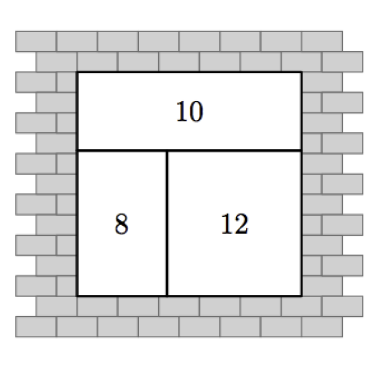
\includegraphics[width=0.4\textwidth]{ЭлМШ 2025-2026/I блок/7/1.3.1.png}
\end{center}

\problem{2}
Комендант измерил периметры всех комнат в доме и написал их на плане. В одну комнату он не сумел попасть, зато обошёл дом кругом и нашел, что его периметр равен $85 м$. Чему равна толщина стен в доме, если она везде одинакова?

\begin{center}
    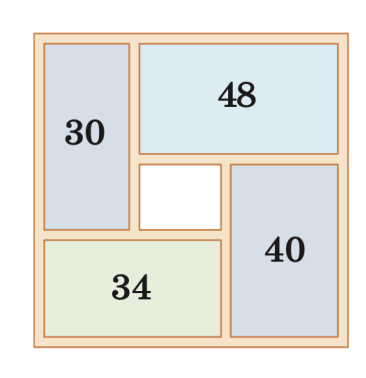
\includegraphics[width=0.4\textwidth]{ЭлМШ 2025-2026/I блок/7/1.4.1.png}
\end{center}